\section{Results}

\begin{itemize}
    \item Methods on how we're doing simulations and results (with simulations and experimental data)
    \begin{itemize}
        \item Different SNRs and maybe even use CAPs
        \item Selection of HRF explained if both use the same but it's different from what's used for simulating.
        \begin{itemize}
            \item What happens? For example with gamma for simulating.
        \end{itemize}
        \item Selection of regularization parameter
        \begin{itemize}
            \item Present with real data on a voxel
        \end{itemize}
    \end{itemize}
\end{itemize}

A critical decision with deconvolution methods is the selection of the regularization parameter \(\lambda\), for which many techniques have been proposed in the literature; but an optimal is yet to be discovered. In fact, Paradigm Free Mapping and Total Activation base their selection of the regularization parameter on different criteria: the Bayesian Information Criterion (BIC)~\cite{schwarz1978estimating} and Akaike Information Criterion (AIC)~\cite{akaike1998information}, and a selection based on the convergence of the residuals to a pre-estimated level of the noise respectively. Hence, we compare the performance of the two algorithms with both selection criteria. Furthermore, we explore the differences between the techniques in terms of the estimation of the activity-inducing signal \(\mathbf{s}\) using the \textit{spike model} in~\eqref{eq:pfm_spike} and the innovation signal \(\mathbf{u}\) using the \textit{block model} in~\eqref{eq:pfm_block}.

\subsection{Simulated and experimental data}

In order to compare the two methods while controlling for their correct performance, we simulated a 400 seconds (TR = 2 s) time series with five neuronal events and we added noise of different sources (physiological, thermal and motion-related) with different signal-to-noise ratios (SNR = [20 dB, 10 dB, 3 dB]) that represent low, medium and high levels of noise as shown in Figure~\ref{fig:simulations}.

\begin{figure}[h]
    \begin{center}
        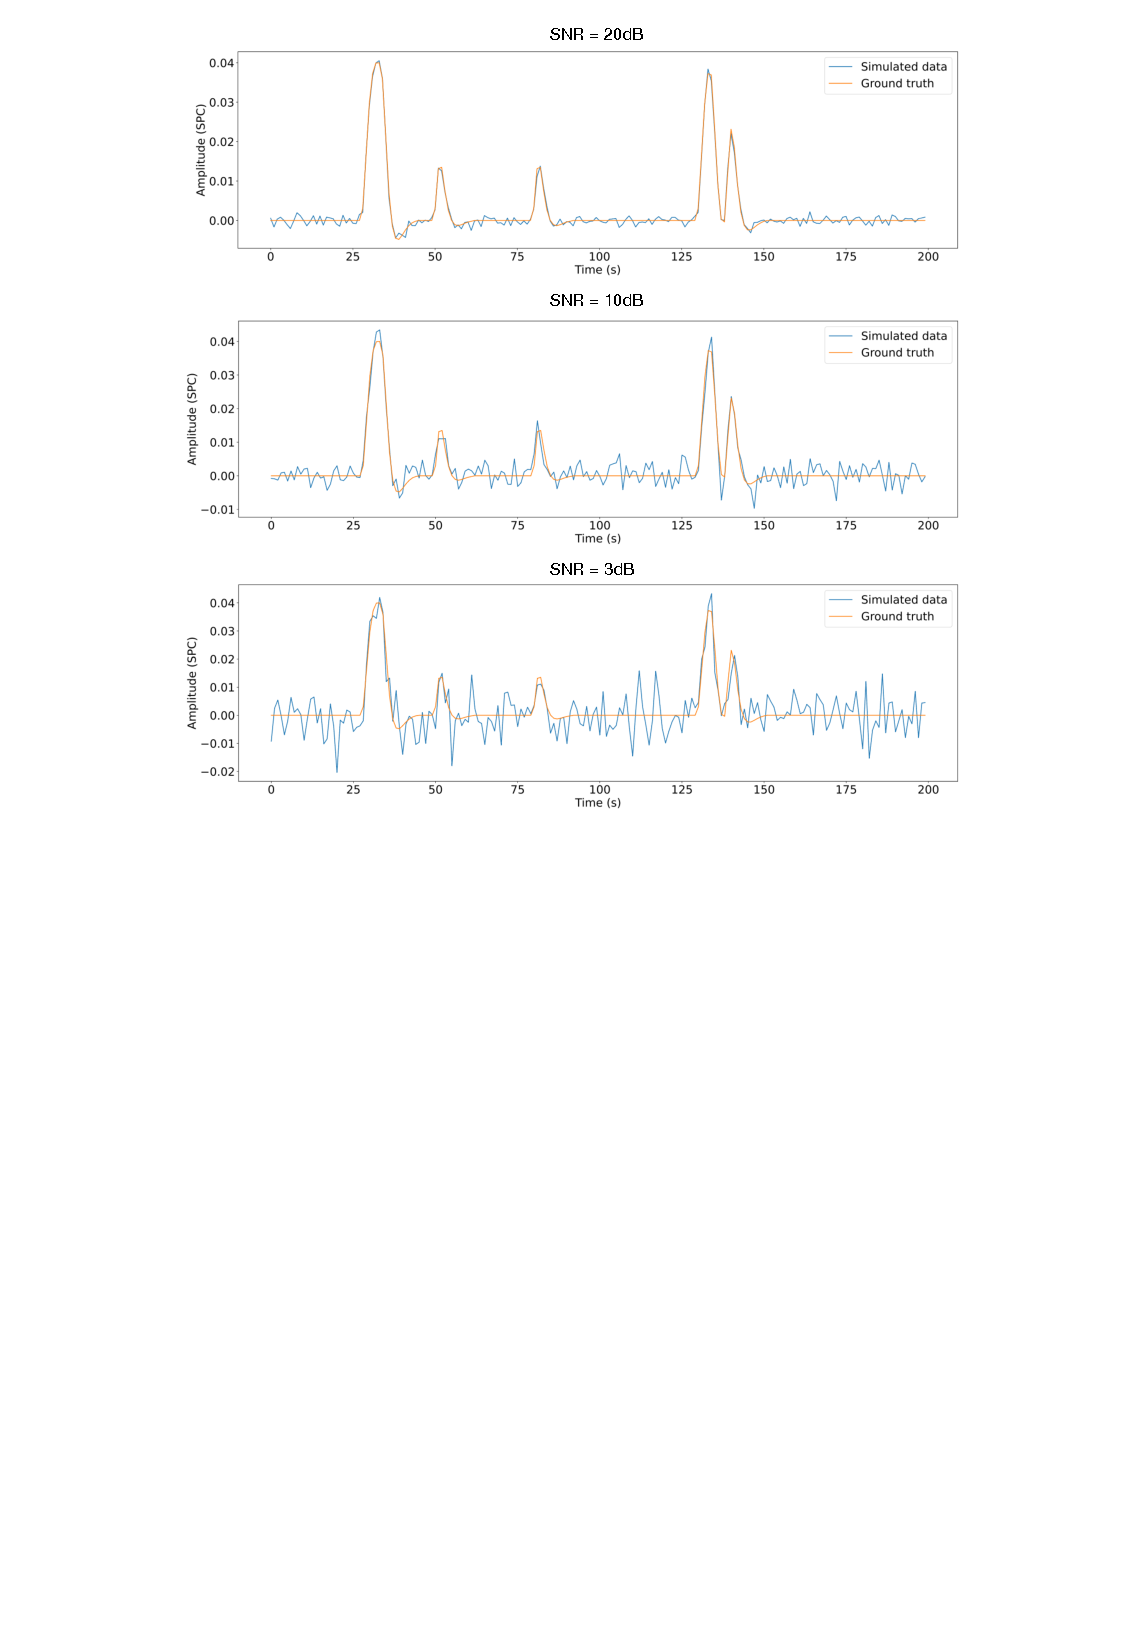
\includegraphics[width=\columnwidth]{figures/sim.pdf}
    \end{center}
    \caption{Simulated signal with different SNRs (20 dB, 10 dB and 3 dB).}
\label{fig:simulations}
\end{figure}

Furthermore, we compared the two techniques on a finger-tapping task where the ground-truth is unknown. For this comparison, we selected a voxel that best represented the finger-tapping paradigm described in~\cite{urunuela2020stability} as shown in Figure~\ref{fig:finger_tapping}.

\begin{figure}[h]
    \begin{center}
        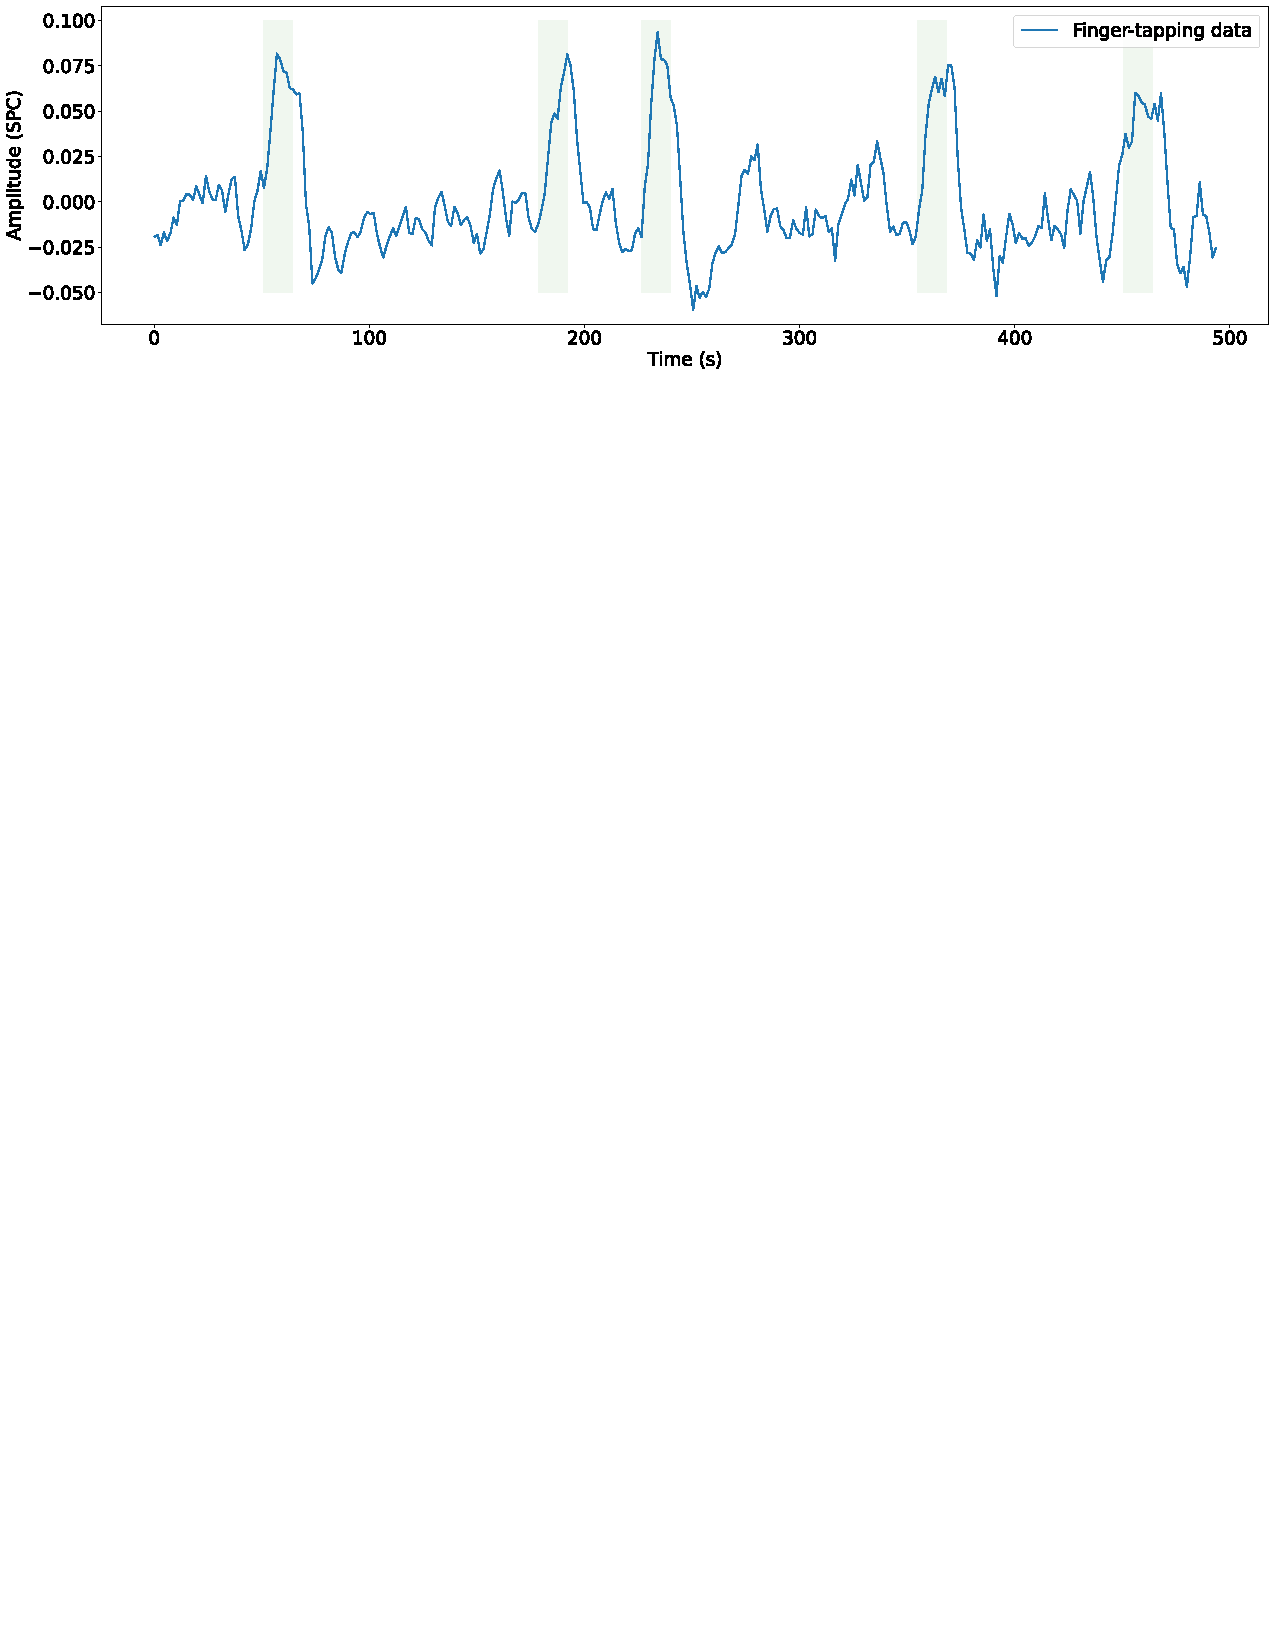
\includegraphics[width=\columnwidth]{figures/finger_tapping.pdf}
    \end{center}
    \caption{Most representative voxel of the finger-tapping task. Green blocks indicate the onsets and the duration of it.}
\label{fig:finger_tapping}
\end{figure}

\subsection{Selection of the hemodynamic response function}

With the aim of making a fair comparison of the two methods, we first compared their hemodynamic response functions. Figure~\ref{fig:hrf_diff} shows the difference in the hemodynamic response function that PFM and TA use by default; the SPMG1 and the HRF resulting from the linear differential operator respectively. A clear difference is observable in that the PFM hemodynamic response function begins at zero while the TA HRF starts at 1. Hence, the Total Activation HRF starts close to its peak, which is advanced around 2.5 frames with respect to PFM. Another difference worth mentioning is that PFM normalizes its HRF to a peak amplitude of 1, whereas the TA HRF is not normalized.

\begin{figure}[h]
    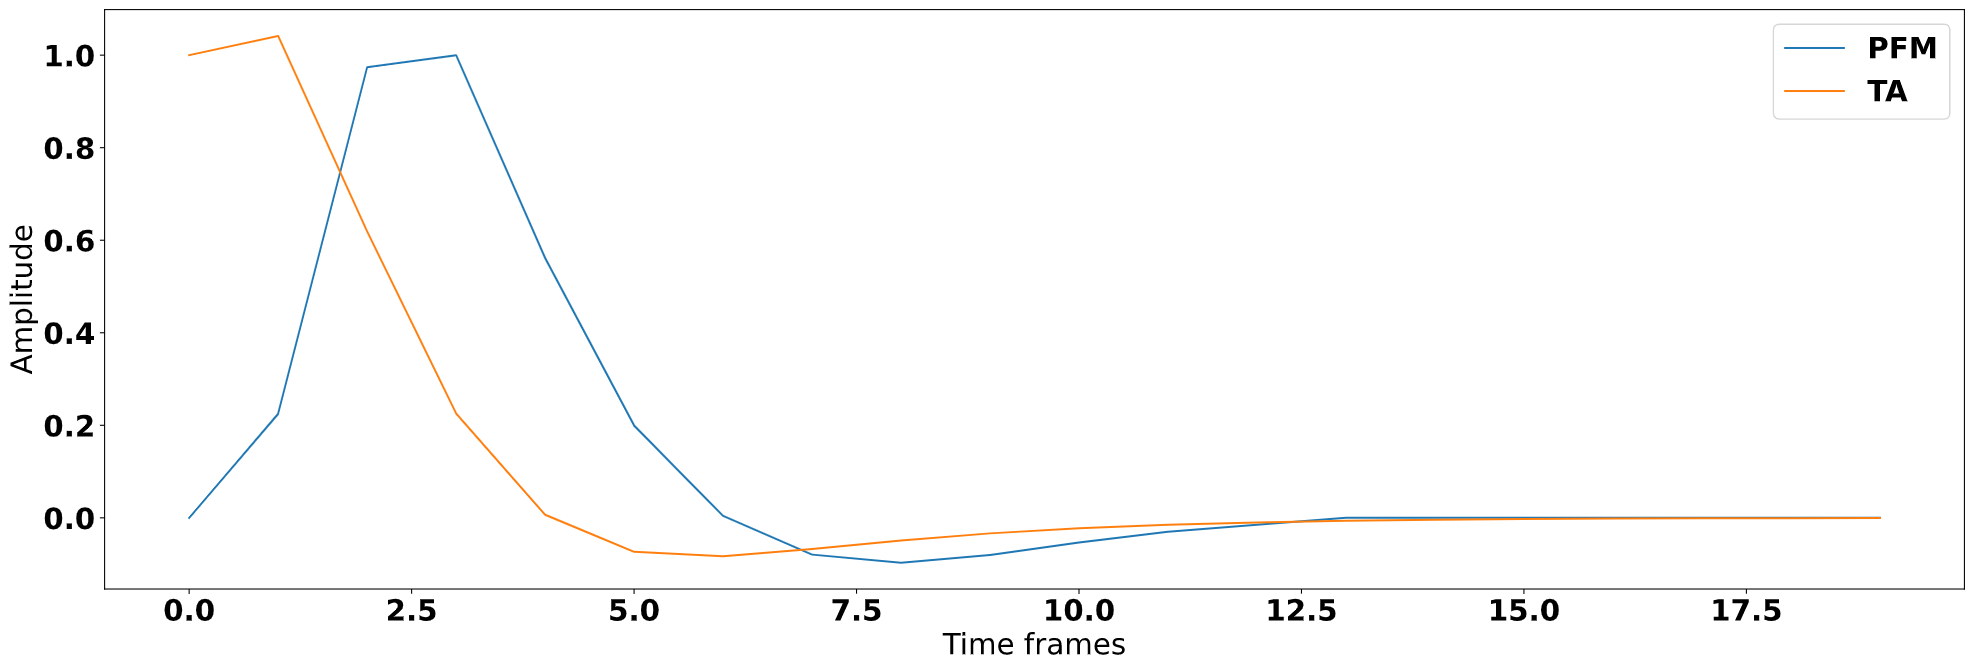
\includegraphics[width=\columnwidth]{figures/hrf_diff.png}
    \caption{Diffence in the HRF of PFM (blue) and TA (orange).}
\label{fig:hrf_diff}
\end{figure}

While Paradigm Free Mapping allows for the use of any hemodynamic response function --- the columns of the design matrix \(\mathbf{H}\) are composed by shifted versions of the HRF --- the linear differential operator in TA is tailored for a fixed HRF. Hence, for practical reasons, we reproduced the HRF in the Total Activation filter and incorporated it into the PFM formulation.

\subsection{Selection of the regularization parameter based on the estimation of the noise}

Total Activation proposes to solve the inverse problem by updating the regularization parameter \(\lambda\) on every iteration \(n\) so that the residuals converged to a previously estimated noise level of the data fit \(\tilde{\sigma}\), where the pre-estimated noise level is calculated from the median absolute deviation of fine-scale wavelet coefficients (Daubechies, order 3)~\cite{karahanouglu2013total}:

\begin{equation}
    \lambda^{n+1} = \frac{N \tilde{\sigma}}{\frac{1}{2} \| \mathbf{y} - \mathbf{x}^n \|_F^2} \lambda^n
\end{equation}

\subsection{Selection of the regularization parameter by solving the regularization path}

\begin{figure*}[t!]
    \begin{center}
        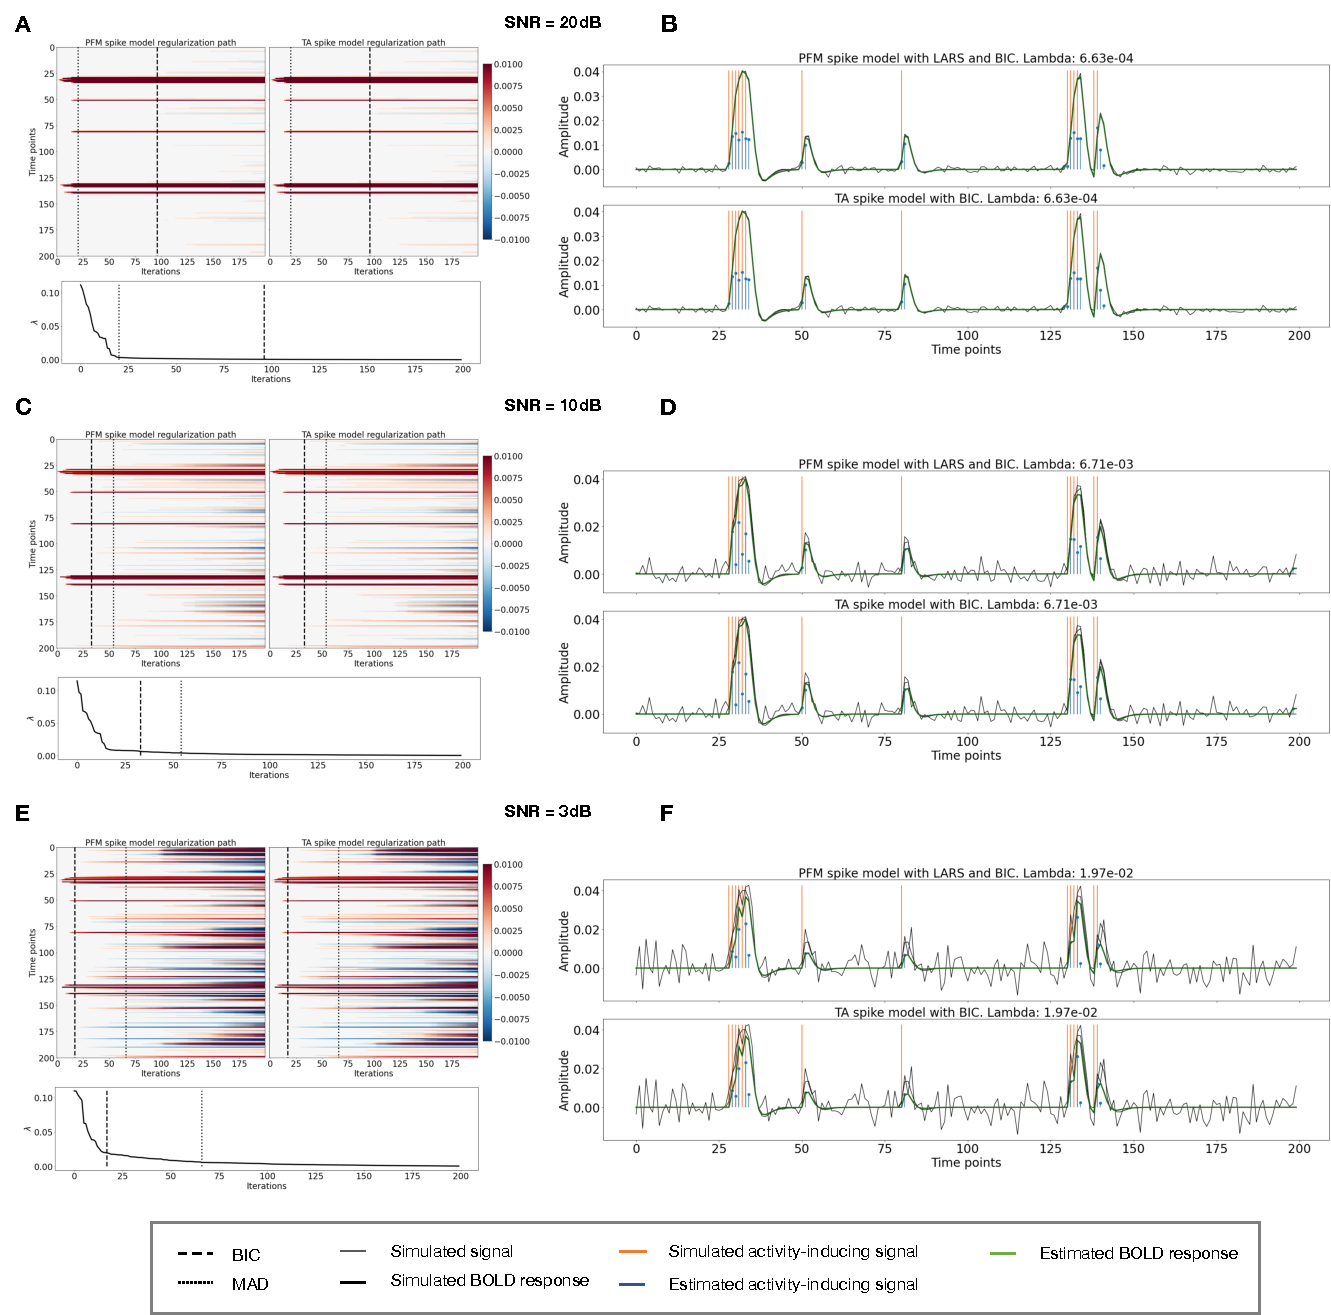
\includegraphics[]{figures/regpath_spike.pdf}
    \end{center}
    \caption{Regularization path and estimated activity-inducing and neuronal-related signals with the spike model and a selection of \(\lambda\) based on BIC. Each row of plots corresponds to a different SNR condition.}
\label{fig:path_spike}
\end{figure*}

\begin{figure*}[t!]
    \begin{center}
        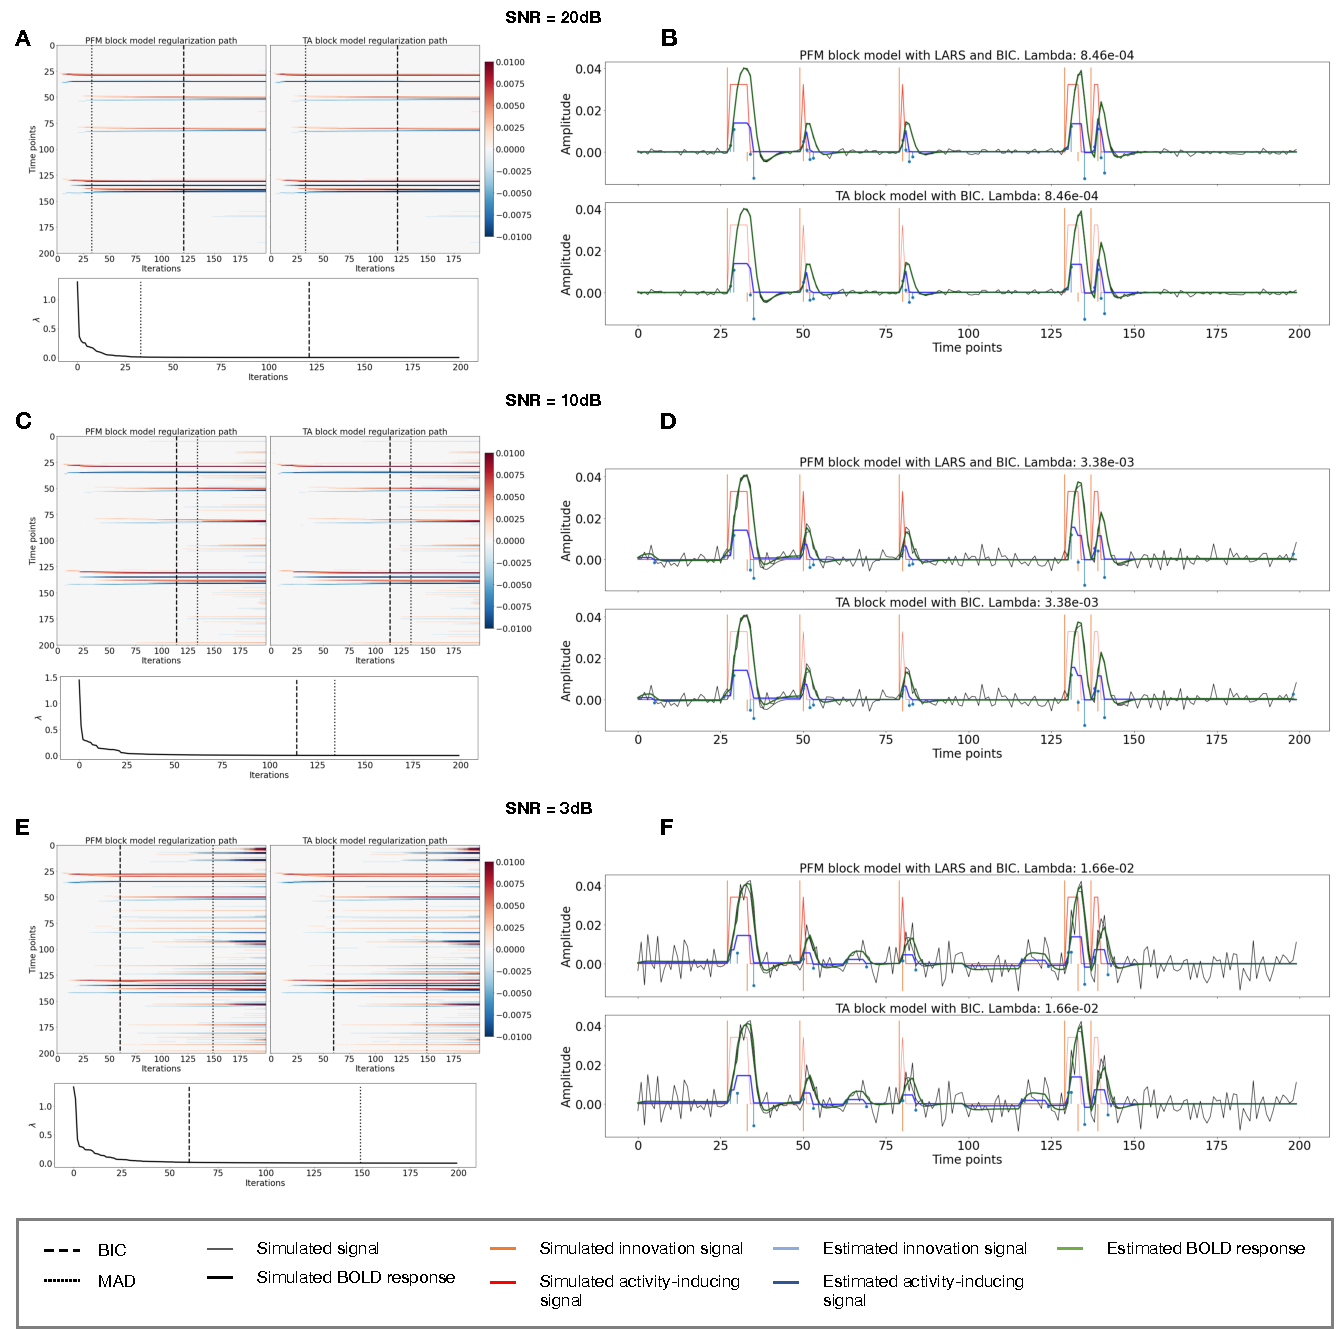
\includegraphics[]{figures/regpath_block.pdf}
    \end{center}
    \caption{Regularization path and estimated activity-inducing and neuronal-related signals with the block model and a selection of \(\lambda\) based on BIC. Each row of plots corresponds to a different SNR condition.}
\label{fig:path_block}
\end{figure*}

Paradigm Free Mapping bases its selection of the regularization parameter on the Bayesian Information Criterion (BIC)~\cite{schwarz1978estimating} and the Akaike Information Criterion (AIC)~\cite{akaike1998information}. Hence, we calculated the entire regularization path with PFM by means of the least angle regression (LARS) algorithm~\cite{efron2004least} and used the \(\lambda\) in the path to solve the deconvolution problem with Total Activation. 

Figure~\ref{fig:path_spike} (left) shows the regularization path of PFM and TA side by side for the three SNR conditions for the spike model; i.e., the inverse problem described in~\eqref{eq:pfm_spike}. Each iteration of LARS reduces the value of \(\lambda\); i.e., reduces the sparsity promoted by the \(l_1\)-norm, and reveals a new non-zero coefficient as shown in the x axis of the heatmaps. Vertical black lines depict the selection of the regularization parameter based on BIC and AIC, and thus, the colored coefficients to the left of the vertical lines depict the estimated activity-inducing signal \(s(t)\). Figure~\ref{fig:path_spike} (right) illustrates the resulting estimation of the activity-inducing and neuronal-related signals when basing the selection of \(\lambda\) on BIC for the three simulated SNR conditions. Given that the regularization paths of both techniques are identical, the BIC-based selection of the regularization parameter and the results of deconvolving with said \(\lambda\) are identical too. Thus, Figure~\ref{fig:path_spike} demonstrates that, regardless of the SNR condition, both deconvolution algorithms produce identical regularization paths when the same HRF and regularization parameters are applied, and hence, identical estimates of the activity-inducing signal \(\mathbf{s}\) and neuronal-related signal \(\mathbf{x}\).

The regularization path to estimate innovation signals; i.e., solving the optimization problem using the block model in~\eqref{eq:pfm_block}, yields identical results for both PFM and TA methods as shown in Figure~\ref{fig:path_block} (left). Again, the BIC-based selection of \(\lambda\) is identical for both PFM and TA and the estimation of the innovation signal \(\mathbf{u}\) shows no distinguishable differences between the algorithms (see Figure~\ref{fig:path_block} right). Therefore, both Paradigm Free Mapping and Total Activation yield identical regularization paths and estimates of the innovation signal regardless of the SNR condition when applying the same HRF and regularization parameters with the block model.
